\chapter{Translation Pipeline} \label{chap:pipeline}
In this chapter, I evaluate the ability of large language models (LLMs) to translate Linear B into Ancient Greek. 
The full pipeline proceeds as follows:

\begin{itemize}[leftmargin=2em]
  \item \textbf{Vocabulary extraction.} Gather every distinct word form attested in the Linear B documents (after cleaning/normalization).
  \item \textbf{Brute-force cognates.} For forms not already covered by our dataset, run the brute-force search against the Ancient Greek lexicon to obtain initial candidates (detailed in Section \ref{sec:bruteforce-cognates}).
  \item \textbf{Candidate aggregation.} For each word, collect possible cognates from: (i) the dataset's suggested cognates, (ii) the raw output of the cognate-matching model trained on our dataset, together with the output of all decoding modes, and (iii) a version of the cognate matcher retrained on the enlarged set. Duplicates are removed from the candidate set.
  \item \textbf{Auxiliary signals.} Train the Linear-SVM auxiliary classifiers on their labeled sets, then predict part of speech, noun type, and inflection for every word in the corpus.
  \item \textbf{Logograms.} Map logograms to their conventional readings/values and include these as fixed translations.
  \item \textbf{LLM prompting.} For each item, assemble a structured prompt containing: the Linear B form, the deduplicated cognate candidates, auxiliary predictions, and relevant morphological guidance. The LLM is asked to (a) select or propose the most plausible Ancient Greek reconstruction, and (b) provide an English translation.
  If the information provided with the prompt is sufficient, the LLM should be able to reconstruct the right inflection for each term and disambiguate the sentence.
\end{itemize}

\begin{figure}[H]
    \begin{adjustbox}{center}
        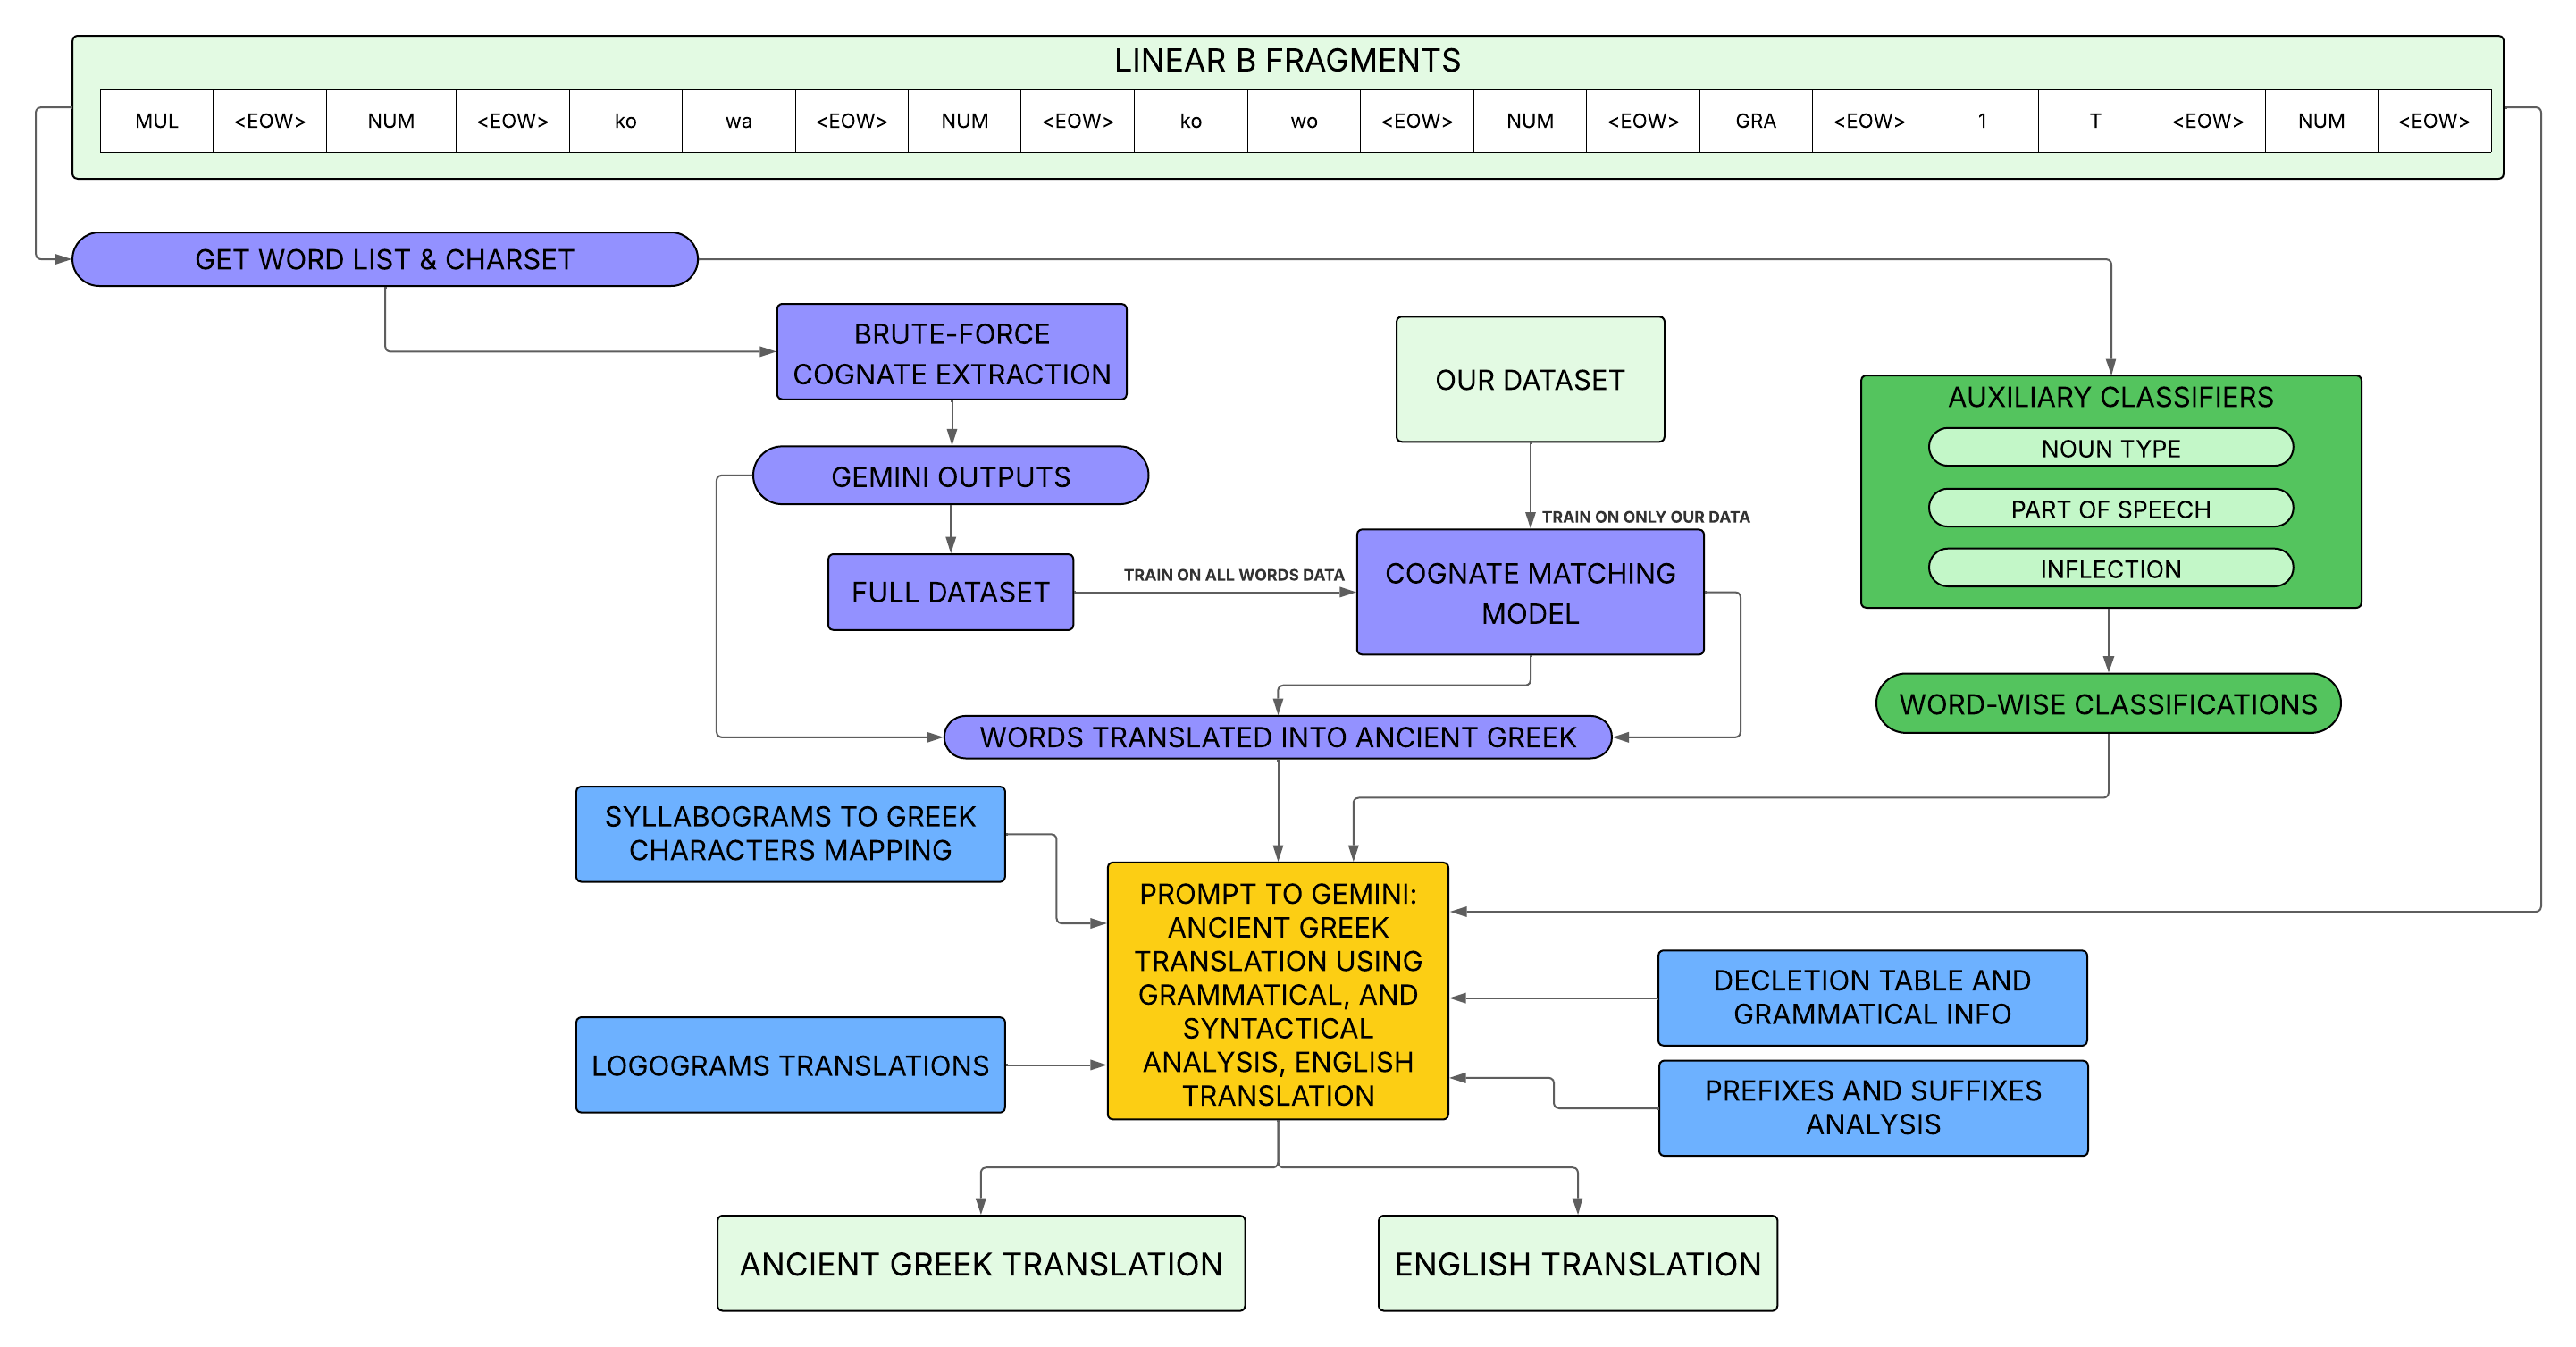
\includegraphics[width=1.2\textwidth]{images/pipeline.png}
    \end{adjustbox}
    \caption{Overview of the translation pipeline from Linear B to Ancient Greek.}
    \label{fig:pipeline}
\end{figure}

\section{Prompt Design} \label{sec:final-prompt}
This time, instead of a single prompt, the information was given to the large language model using a series of structured messages, each with a specific role.

\paragraph{Historical Context}
The first message provided to the model was a simple historical context on Linear B and Ancient Greek relationship.
It underlines the fact that Linear B is an early form of Greek, written with a syllabic script, and its administrative nature.
This message was fixed for all words.

\paragraph{Syllabogram Matching}
The second message contained the Linear B syllabograms and their closest Ancient Greek equivalents, predicted by Luo's model.
It associates to each Linear B syllabogram a list of symbols that could represent it in its Ancient Greek correspondence.
For example, the Linear B syllabogram \textlinb{\Bpa} (pa) is associated with the Ancient Greek letters \textgreek{π}, \textgreek{φ}, and \textgreek{α}, as it usually corresponds to "\textgreek{πα}" or "\textgreek{φα}" syllables.
This was also fixed for all words.

\paragraph{Grammatical Information}
The third message provided auxiliary grammatical information, such as Linear B declension tables, and additional information about adjectives and verbs, like in the prompt described in Section \ref{sec:aux-dataset}.

\paragraph{Task Definition}
The fourth message formalizes the task. The model receives the Linear~B document as a sequence of tokenized word forms; for each word it is given (i) the aggregated set of candidate Ancient Greek cognates, (ii) auxiliary predictions (part of speech, noun type when applicable, and inflection when applicable), and (iii) a completeness label.
The completeness label is derived from the share $p\!\in\![0,1]$ of occurrences marked as "complete" in the corpus and is bucketed at fixed cutoffs:
\emph{Always Complete} ($p=1$), \emph{Mostly Complete} ($p \geq \frac{2}{3}$), \emph{Uncertain} ($\frac{1}{3} < p < \frac{2}{3}$), \emph{Mostly Incomplete} ($0< p \leq \frac{1}{3}$), \emph{Incomplete} ($p=0$).

The prompt instructs the model on how to complete the translation task, the main steps being:
\begin{itemize}
  \item \textbf{Grammatical analysis.} The first step is to analyze the grammatical features of the Linear B document, separating the words into adjectives, nouns, verbs, and adverbs, and reconstructing the inflection of each noun and adjective, as well as the conjugation of each verb.
  \item \textbf{Syntactic analysis.} The second step is to analyze the document's structure by identifying its sentences and distinguishing the subjects, verbs, and objects mentioned in them.
  \item \textbf{Discourse analysis.} The third step is to analyze the discourse, examining subordinate clauses and establishing coherent logical connections.
  \item \textbf{Linguistic authenticity.} The fourth step is to ensure the selection of an Ancient Greek cognate that preserves morphological patterns and is plausible given the corresponding Mycenaean Greek form.
  \item \textbf{Semantic coherence.} The last step is to ensure that the translation is semantically coherent with the administrative nature of the Linear B documents.
\end{itemize}

These are common steps in translation and linguistic analysis, but they are particularly important in this context due to the similarity between Linear B inflected forms.
The LLM is finally asked given some quality assurance criteria, reflecting the needs of the task, and instructed to use the chain-of-thought technique to reason step by step and refine its translation.

\paragraph{Examples}
The last information given to the model is a series of examples of translated Linear B fragments.
These examples are selected from a small set of documents provided by Chris Tselentis, together with his Linear B lexicon \cite{tselentis}.

These examples are very short, but they cover a variety of linguistic phenomena and be representative of the administrative purpose of the documents.
The following examples were used:

\begin{enumerate}
  \item \textbf{PY Eb 895+906}: This brief document contains a subordinate clause introduced by a participial form.
  Therefore, it provides key features of Linear B clause structure. \\
  \textbf{Linear B original}: \textlinb{\Ba\Bi\Bqe\Bu} \textlinb{\Be\Bke\Bqe} \textlinb{\Bke\Bke\Bme\Bna} \textlinb{\Bko\Bto\Bna} \textlinb{\Bko\Bto\Bno\Bko} \textlinb{\Bto\Bso\Bde} \textlinb{\Bpe\Bmo} \textlinb{\BPwheat} \textlinb{\BPvolcd} \textlinb{\BNvi}\\
  \textbf{Linear B text}: a-i-qe-u e-ke-qe ke-ke-me-na ko-to-na ko-to-no-o-ko to-so-de pe-mo GRA T 6 \\
  \textbf{Greek translation}: \textgreek{Αἰγεὺς κτοινόοχος ἔχει τε κεκειμένα κτοίνα τοσόνδε σπέρμον ΣΙΤΟΣ Τ 6} \\
  \textbf{English translation}: Aigeus, the plot owner, who owns a communal plot; so much grain: 6 'T' units of wheat. \\
  
  \begin{figure}[H]
    \centering
    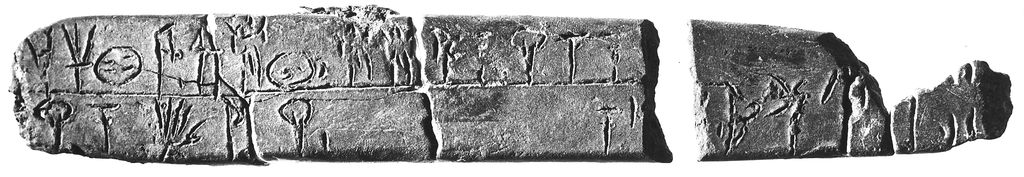
\includegraphics[width=0.7\textwidth]{Images/4901.png} % Adjust width and filename
    \caption{Picture of the original document PY Eb 895+906.}
    \label{fig:example1}
  \end{figure}

  \item \textbf{PY Ta 711}: This fragment is very short as well. It is excerpted from a longer document, whose translation will be fully evaluated in Section \ref{sec:translations}.
  However, it also contains a subordinate clause, introduced here by a particle.
  Moreover, it underscores the importance of grammatical and syntactic analysis, as the subject and the object of the sentence exhibit overlapping inflectional endings. \\
  \textbf{Linear B original}: \textlinb{\Bo\Bwi\Bde} \textlinb{\Bpu\Bke\Bqi\Bri} \textlinb{\Bo\Bte} \textlinb{\Bwa\Bna\Bka} \textlinb{\Bte\Bke} \textlinb{\Bau\Bke\Bwa} \textlinb{\Bda\Bmo\Bko\Bro}\\
  \textbf{Linear B text}: o-wi-de phu-ke-qi-ri o-te wa-na-ka te-ke au-ke-wa da-mo-ko-ro \\
  \textbf{Greek translation}: \textgreek{ὀ-εἶδε Φυγεκλής ὅτε ἄναξ θῆκε Αὐγέαν δάμοκλον} \\
  \textbf{English translation}: Phygekles witnessed when the king appointed Augeus as damoklos. \\

  \begin{figure}[H]
    \centering
    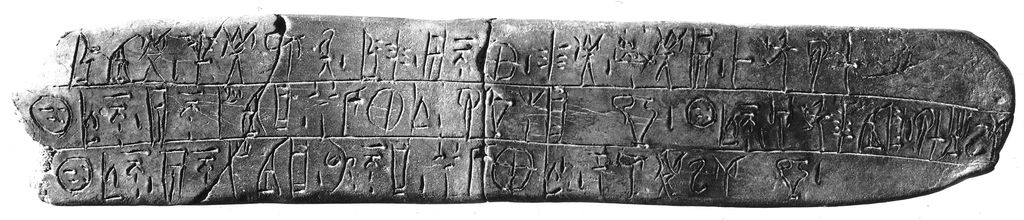
\includegraphics[width=0.8\textwidth]{Images/5350.png} % Adjust width and filename
    \caption{Picture of the original document PY Ta 711.}
    \label{fig:example2}
  \end{figure}

  \item \textbf{PY Ae 303}: This very brief document, like the previous two, illustrates long-distance agreement: the attributive adjective and the noun it modifies stand far apart in the line.
This word-order freedom is common in Ancient Greek and underscores why careful grammatical and logical analysis is essential. \\
  \textbf{Linear B original}: \textlinb{\Bi\Bje\Bro\Bjo} \textlinb{\Bpu\Bro} \textlinb{\Bi\Bje\Bre\Bja} \textlinb{\Bdo\Be\Bra} \textlinb{\Be\Bne\Bka} \textlinb{\Bku\Bru\Bso\Bjo} \textlinb{\BPwoman} \textlinb{\BNx\BNiv}\\
  \textbf{Linear B text}: i-je-ro-jo pu-ro i-je-re-ja do-e-ra e-ne-ka ku-ru-so-jo MUL 14 \\
  \textbf{Greek translation}: \textgreek{Πύλος: ιερείας δούλαι ένεκα χρυσοίο ιεροίο ΓΥΝΗ 14} \\
  \textbf{English translation}: Pylos: slaves of the priestess for the sake of sacred gold, 14 women. \\

  \begin{figure}[H]
    \centering
    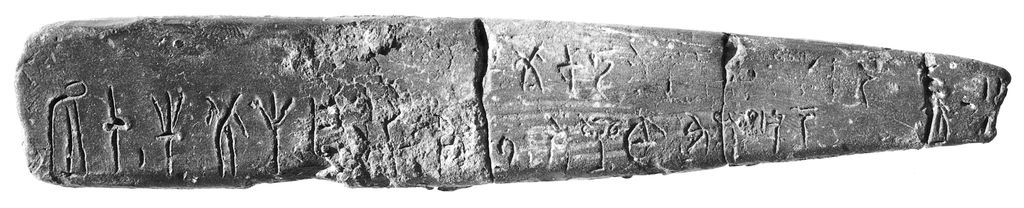
\includegraphics[width=0.7\textwidth]{Images/4684.png} % Adjust width and filename
    \caption{Picture of the original document PY Ae 303.}
    \label{fig:example3}
  \end{figure}

\end{enumerate}

\paragraph{Outputs}
The model is expected to output a JSON object with three fields:
\begin{itemize}
  \item \texttt{Ancient Greek}: the reconstructed Ancient Greek translation of the Linear B document.
  \item \texttt{English}: the English translation of the Linear B document.
  \item \texttt{Reasoning}: a detailed reasoning process, following the steps outlined in the task definition, explaining how the model arrived at its translations.
\end{itemize}

\section{Results} \label{sec:translations}
In this section, the outputs of the Translation Pipeline will be presented and compared with existing translations of the same documents, provided by Tselentis' lexicon \cite{tselentis}.

The parameters used for the LLM are the following: Gemini~2.5~Flash, with temperature 0.1, top-p 0.95, and top-k 0.4.

The evaluation will focus on the quality of the Ancient Greek reconstructions and the accuracy of the English translations.
Moreover, errors will be analyzed and the reasoning provided by the model will be assessed to understand the possible causes of mistakes.
A small sample of documents will not be assessed, as it was used as examples in the prompt (see Section \ref{sec:final-prompt}).

\subsection{Evaluated Documents}
The documents selected for evaluation are the following:
\begin{enumerate}[label=(\roman*)]
\item PY Ta 711
\item KN Ra 1540
\item PY Jn 310
\item PY Jn 829
\item KN So 4439
\item KN Sd 4404
\item PY An 657
\item PY TA 641
\item PY Er 312
\item KN Fp 1+31
\item PY Ab 573
\item PY Un 718
\end{enumerate}

The fragments of the documents whose translations were provided by Tselentis are highlighted in \emph{italics}.

\subsubsection{PY Ta 711}
This document was already presented as part of the examples in the prompt to the LLM.
However, only the first fragment was used as an example, while the rest of the document was reserved for evaluation. \\
\textbf{Linear B text}: \textit{o-wi-de phu-ke-qi-ri o-te wa-na-ka te-ke au-ke-wa da-mo-ko-ro} qe-ra-na wa-na-se-wi-ja qo-u-ka-ra ko-ki-re-ja *204VAS 1 qe-ra-na a-mo-te-wi-ja ko-ro-no-we-sa qe-ra-na wa-na-se-wi-ja ku-na-ja qo-u-ka-ra 1 to-qi-de-we-sa *204VAS 1 \\
\textbf{Greek translation}: \textgreek{ὀ-εἶδε Φυγεκλής ὅτε ἄναξ θῆκε Αὐγέαν δάμοκλον. κερανα ϝανασεϝια βουκαρα κοχλιρεια ΣΚΕΥΟΣ 1. κερανα αρμοθηϝια κορωνοϝέσσα. κερανα ϝανασεϝια γυναια βουκαρα 1. τροπιδϝέσσα ΣΚΕΥΟΣ 1.} \\
\textbf{English translation}: Phygekles witnessed when the king appointed Augeus as damoklos. A royal, ox-head-shaped, spiral-decorated krater (vessel): 1. A krater with fittings, with a handle. A royal, female, ox-head-shaped krater: 1. A spiral-designed vessel: 1.

\paragraph{Analysis.}
After the first narrative clause, the document lists four types of vessels.
The LLM correctly reconstructs the context and provides a meaningful and coherent translation.

Let's analyze the four vessel descriptions in detail:
\begin{itemize}
\item The word \textlinb{\Bqe\Bra\Bna} (qe-ra-na) is correctly identified as a noun, and the LLM selects the Ancient Greek cognate \textgreek{κερανα}.
However, the expected form would definitely be \textgreek{κέρνα}, the nominative/accusative plural of \textgreek{κέρνος}, which is used in Ancient Greek to denote a sacred vessel.
\item The word \textlinb{\Bwa\Bna\Bse\Bwi\Bja} (wa-na-se-wi-ja) is correctly identified as an adjective, and the LLM selects an Ancient Greek form that closely echoes the original Linear B word: \textgreek{ϝανασεϝια}, rather than the Ancient Greek \textgreek{αναξια}.
Other adjectives referring to this vessel are \textlinb{\Bqo\Bu\Bka\Bra} (qo-u-ka-ra, "ox-head shaped") and \textlinb{\Bko\Bi\Bre\Bja} (ko-ki-re-ja, "spiral-decorated").
The first is associated with a synthetic compound Ancient Greek form composed of \textgreek{βους} "ox" and \textgreek{καρα} "head", while the second is translated as \textgreek{κοχλιρεια}, an adjective derived from \textgreek{κοχλος}, "spiral-shaped shell", sharing the root with Ancient Greek \textgreek{κοχλιοειδης/κοκλιωδης}.
\item The following vessel is associated with the adjectives \textlinb{\Bko\Bro\Bno\Bwe\Bsa} (ko-ro-no-we-sa), meaning the krater is provided with handles (from Ancient Greek \textgreek{κορωνη}), and \textlinb{\Ba\Bmo\Bte\Bwi\Bja} (a-mo-te-wi-ja), linked to the concept of "fittings" or chariot-related terms (from Ancient Greek \textgreek{αρμος} "joint" and \textgreek{αρμα} "chariot"), even though no fully satisfactory Greek correspondence can be found.
\item The third vessel is again described as royal and ox-head shaped, but the third adjective is \textlinb{\Bku\Bna\Bja} (ku-na-ja), from Ancient Greek \textgreek{γυναια}, "womanly".
\item The last vessel is described as \textlinb{\Bto\Bqi\Bde\Bwe\Bsa} (to-qi-de-we-sa), "spiral-designed", from Ancient Greek \textgreek{τροπιδϝέσσα}, derived from \textgreek{τροπις}, which actually means "keel", and whose connection to spirals is only indirect through the notion of turning or curving, but is also confirmed by Tselentis' lexicon \cite{tselentis}.
\end{itemize}
Overall, the LLM's English translation is quite accurate, while the Ancient Greek reconstruction still retains Linear B features.

Here I report an improved version of the Greek translation, highlighting in red the adjustments. For the English translation, no changes are needed. \\
\textbf{Greek translation}: \textcolor{red}{\textgreek{οἶδε}} \textgreek{Φυγεκλής ὅτε ἄναξ θῆκε Αὐγέαν δάμοκλον.} \textcolor{red}{\textgreek{κέρνα ἀναξία}} \textgreek{βουκάρα} \textcolor{red}{\textgreek{κοχλιοειδή}} \textgreek{ΣΚΕΥΟΣ 1.} \textcolor{red}{\textgreek{κέρνα}} \textgreek{αρμοθήϝια κορωνοϝέσσα}. \textcolor{red}{\textgreek{κέρνα ἀναξία}} \textgreek{γυναίκα βουκάρα 1. τροπιδϝέσσα ΣΚΕΥΟΣ 1.}

The picture of this document is shown in Figure \ref{fig:example2}.

\subsubsection{KN Ra 1540}
This document is a very short inventory entry of a single item: swords. \\
\textbf{Linear B text}: \textit{to-sa pa-ka-na PUG 50} \\
\textbf{Greek translation}: \textgreek{τόσα φάσγανα ΦΑΣΓΑΝΑ 50.} \\
\textbf{English translation}: So many swords: 50 SWORDS.
\paragraph{Analysis.}
In this case, the LLM correctly reconstructs the whole document, due to its simplicity.
The words \textlinb{\Bto\Bsa} (to-sa) and \textlinb{\Bpa\Bka\Bna} (pa-ka-na) are correctly identified as a quantifier and a noun, respectively.
They are translated into their corresponding Ancient Greek cognates: \textgreek{τόσα} and \textgreek{ϝάσγανα}, the accusative plural of \textgreek{ϝάσγανον}, "sword".
The English translation is also accurate, therefore no changes are needed.

\begin{figure}[H]
  \centering
  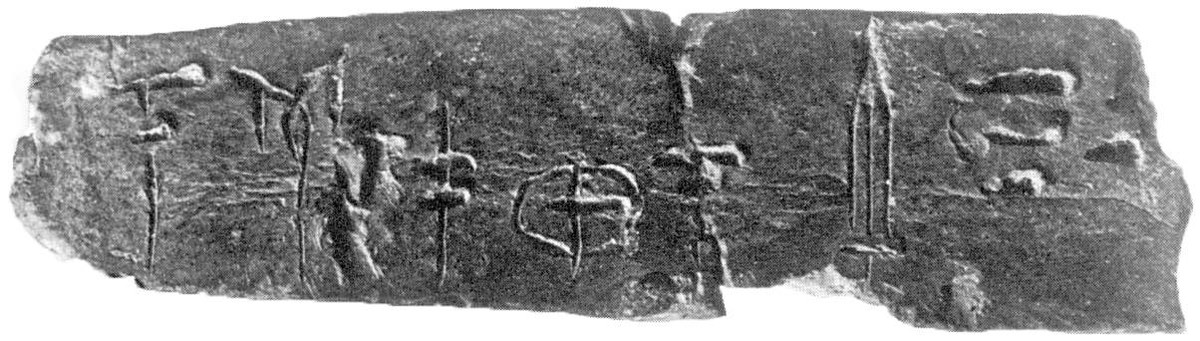
\includegraphics[width=0.7\textwidth]{Images/250.png} % Adjust width and filename
  \caption{Picture of the original document KN Ra 1540.}
  \label{fig:doc2}
\end{figure}

\subsubsection{PY Jn 310}
Tselentis provides a translation for only a fragment of this document, which is quite long.
However, the LLM appears able to handle the entire text quite well, thanks to its repetitive structure. \\
\textbf{Linear B text}: a-ke-re-wa [...] ka-ke-we ta-ra-si-ja e-ko-te ti-qa-jo AES M 1 N 2 qe-ta-wo AES M 1 N 2 ai-so-ni-jo AES M 1 N 2 ta-mi-je-u AES M 1 N 2 e-u-ru-wo-ta AES M 1 N 2 e-u-do-no AES M 1 N 2 po-ro-u-te-u AES M 1 N 2 wi-du-wa-ko AES M 1 N 2 to-so-de a-ta-ra-si-jo ka-ke-we [...] pa-qo-si-jo 1 ke-we-to 1 [...] 1 [...] pe-ta-ro 1 to-so-de do-e-ro ke-we-to-jo 1 i-wa-ka-o 1 pa-qo-si-jo-jo 1 po-ro-u-te-wo 1 a [...] \textit{po-ti-ni-ja-we-jo ka-ke-we ta-ra-si-ja e-ko-te} i-ma-di-jo [...] AES M 3 tu-ke-ne-u AES M 3 AES M 3 i-wa-ka AES M 3 a-ta-ra-si-jo phu-si-ja-ko 1 \\
\textbf{Greek translation}: \textgreek{Ἀγρεϝα [...] χαλκεϝες ταλανσία ἔχοντες: Τιθαιος ΧΑΛΚΟΣ M 1 N 2, Κεταϝος ΧΑΛΚΟΣ M 1 N 2, Αἰσώνιος ΧΑΛΚΟΣ M 1 N 2, Ταμιεύς ΧΑΛΚΟΣ M 1 N 2, Εὐρυϝότας ΧΑΛΚΟΣ M 1 N 2, Εὔδονος ΧΑΛΚΟΣ M 1 N 2, Πλουτεύς ΧΑΛΚΟΣ M 1 N 2, Ϝιδυϝακος ΧΑΛΚΟΣ M 1 N 2. Τόσοςδε ἀταλανσίοι χαλκεϝες [...]: Παμφίσιος 1, Κηϝετος 1, [...] 1, [...] 1, Πέταλος 1. Τόσοςδε δοῦλοι: Κηϝετοιο 1, Ἰϝακαο 1, Παμφισίοιο 1, Πλουτέϝος 1. Ἀ [...] Ποτνιάϝειοι χαλκεϝες ταλανσία ἔχοντες: Ἱμαδιος [...] ΧΑΛΚΟΣ M 3, Τυχενεύς ΧΑΛΚΟΣ M 3, ΧΑΛΚΟΣ M 3, Ἰϝακα ΧΑΛΚΟΣ M 3. Ἀταλανσίοι: Φυσίαρχος 1.} \\
\textbf{English translation}: Agrewa: [...] bronze-smiths having allotment: Tithaios: BRONZE M 1 N 2, Ketawo: BRONZE M 1 N 2, Aisonios: BRONZE M 1 N 2, Tamieus: BRONZE M 1 N 2, Eurywotas: BRONZE M 1 N 2, Eudonos: BRONZE M 1 N 2, Plouteus: BRONZE M 1 N 2, Widuwako: BRONZE M 1 N 2. Total bronze-smiths without allotment [...]: Pamphisios 1, Kewetos 1, [...] 1, [...] 1, Petalos 1. Total slaves: Of Kewetos 1, Of Iwaka 1, Of Pamphisios 1, Of Plouteus 1. A [...] Potnia-related bronze-smiths having allotment: Himadios [...] BRONZE M 3, Tucheneus: BRONZE M 3, BRONZE M 3, Iwaka: BRONZE M 3. Without allotment: Physiarchos 1.

\paragraph{Analysis.}
This document is an administrative record from the site of Pylos, listing bronze-smiths, their allotments of bronze, and associated personnel (slaves).
It is structured into several sections based on the status and affiliation of the craftsmen.
Most words occurring in the document are proper nouns, for which the Ancient Greek correspondence is a simple transliteration.
The most notable common words are:
\begin{itemize}
\item \textlinb{\Bka\Bke\Bwe} (ka-ke-we), "bronze-smith", from Ancient Greek \textgreek{χαλκεύς}, correctly identified as a noun by the LLM and transliterated in a form preserving the digamma (\textgreek{χαλκεϝες} rather than \textgreek{χαλκεῖς}).
\item \textlinb{\Bta\Bra\Bsi\Bja} (ta-ra-si-ja), "allotment", from Ancient Greek \textgreek{ταλανσία}, also correctly identified as a noun.
It shares its root with \textgreek{τάλαντον}, "talent", a unit of weight (and later currency), with the sense of "allotment" deriving from a weight of metal assigned to a worker.
\item \textlinb{\Be\Bko\Bte} (e-ko-te), "having", from Ancient Greek \textgreek{ἔχοντες}, the nominative plural masculine present active participle of \textgreek{ἔχω}, "to have".
Another straightforward form is \textlinb{\Bdo\Be\Bro} (do-e-ro), from Ancient Greek \textgreek{δοῦλοι}, the nominative plural masculine of \textgreek{δοῦλος}, "slave".
\item Both \textlinb{\Bto\Bso\Bde} (to-so-de) and \textlinb{\Ba\Bta\Bra\Bsi\Bjo} (a-ta-ra-si-jo) are interpreted as nominative plural adjectives referring to the bronze-smiths.
The former means "so many" or "total", from Ancient Greek \textgreek{τοσόσδε}, while the latter means "without allotment", from Ancient Greek \textgreek{ἀταλανσίος}, built from the negative prefix \textgreek{ἀ-} and \textgreek{ταλανσία}, "allotment".
\item The translation of \textlinb{\Bpo\Bti\Bni\Bja\Bwe\Bjo} (po-ti-ni-ja-we-jo) is problematic in this context.
While the LLM interprets it as a nominative plural associated with the bronze-smiths, Tselentis gives it a locative neuter value, linking it to the initial word \textlinb{\Ba\Bke\Bre\Bwa} (a-ke-re-wa), a toponym.
Accordingly, while the LLM's rendering remains vague, Tselentis' proposal is to read it as "at the place of Potnia", associating it with \textgreek{ποτνιάδειον}.
\end{itemize}

The LLM's English translation is quite accurate, although it reflects the issue with the word "po-ti-ni-ja-we-jo".
For both translations, I report an improved version below, highlighting in red the adjustments and in blue the actual mistakes. \\
\textbf{Greek translation}: \textgreek{Ἀγρεϝα [...]} \textcolor{red}{\textgreek{χαλκεῖς}} \textgreek{ταλανσία ἔχοντες: Τιθαιος ΧΑΛΚΟΣ M 1 N 2, Κεταϝος ΧΑΛΚΟΣ M 1 N 2, Αἰσώνιος ΧΑΛΚΟΣ M 1 N 2, Ταμιεύς ΧΑΛΚΟΣ M 1 N 2, Εὐρυϝότας ΧΑΛΚΟΣ M 1 N 2, Εὔδονος ΧΑΛΚΟΣ M 1 N 2, Πλουτεύς ΧΑΛΚΟΣ M 1 N 2, Ϝιδυϝακος ΧΑΛΚΟΣ M 1 N 2.} \textcolor{red}{\textgreek{Τοσοίδε}} \textgreek{ἀταλανσίοι} \textcolor{red}{\textgreek{χαλκεῖς}} \textgreek{[...]: Παμφίσιος 1, Κηϝετος 1, [...] 1, [...] 1, Πέταλος 1.} \textcolor{red}{\textgreek{Τοσοίδε}} \textgreek{δοῦλοι: Κηϝετοιο 1,} \textcolor{red}{\textgreek{Ἰϝακου}} \textgreek{1, Παμφισίοιο 1, Πλουτέϝος 1. Ἀ [...]} \textcolor{blue}{\textgreek{ποτνιάδειον}} \textcolor{red}{\textgreek{χαλκεῖς}} \textgreek{ταλανσία ἔχοντες: Ἱμαδιος [...] ΧΑΛΚΟΣ M 3, Τυχενεύς ΧΑΛΚΟΣ M 3, ΧΑΛΚΟΣ M 3,} \textcolor{red}{\textgreek{Ἰϝακας}} \textgreek{ΧΑΛΚΟΣ M 3. Ἀταλανσίοι: Φυσίαρχος 1.} \\
\textbf{English translation}: Agrewa: [...] bronze-smiths having allotment: Tithaios: BRONZE M 1 N 2, Ketawo: BRONZE M 1 N 2, Aisonios: BRONZE M 1 N 2, Tamieus: BRONZE M 1 N 2, Eurywotas: BRONZE M 1 N 2, Eudonos: BRONZE M 1 N 2, Plouteus: BRONZE M 1 N 2, Widuwako: BRONZE M 1 N 2. Total bronze-smiths without allotment [...]: Pamphisios 1, Kewetos 1, [...] 1, [...] 1, Petalos 1. Total slaves: Of Kewetos 1, Of \textcolor{red}{Iwakas} 1, Of Pamphisios 1, Of Plouteus 1. A [...] \textcolor{blue}{At the place of Potnia}: bronze-smiths having allotment: Himadios [...] BRONZE M 3, Tucheneus: BRONZE M 3, BRONZE M 3, \textcolor{red}{Iwakas}: BRONZE M 3. Without allotment: Physiarchos 1.

\begin{figure}[H]
  \centering
  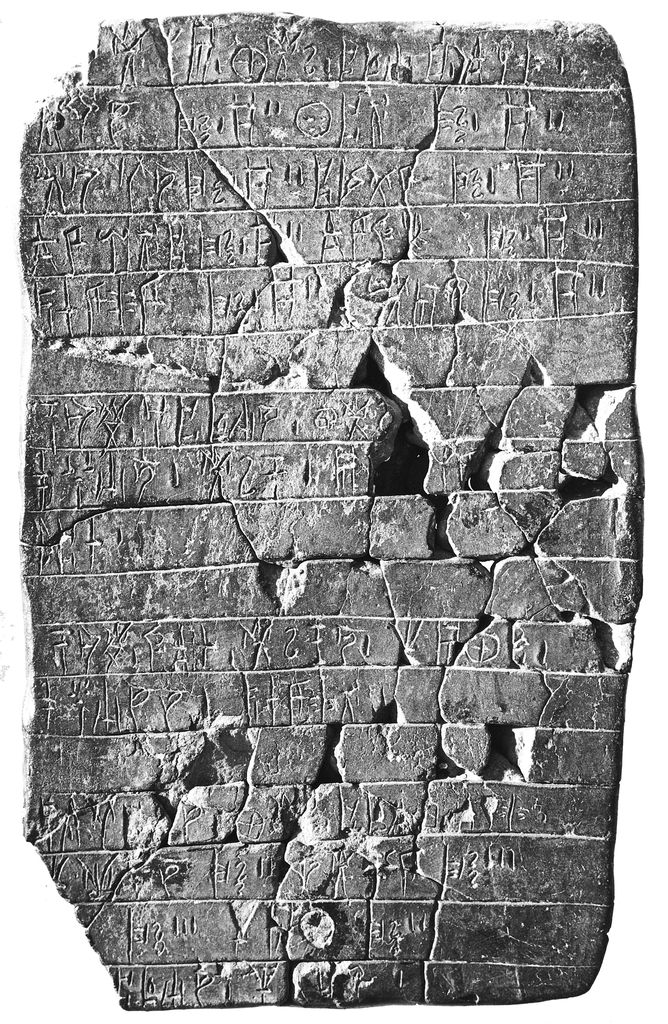
\includegraphics[width=0.55\textwidth]{Images/5057.png} % Adjust width and filename
  \caption{Picture of the original document PY Jn 310.}
  \label{fig:doc3}
\end{figure}

\subsubsection{PY Jn 829}
This document records the quantities of bronze collected for a temple and for the production of arrows.
The opening clause names the givers and states the purpose of the collection.
The remainder lists the amounts of bronze associated with various mayors and deputy mayors.
Because the closing portion is long and highly repetitive, I exclude it from the analysis.
Tselentis’ translation covers only part of the opening sentence. \\
\textbf{Linear B text}: jo-do-so-si ko-re-te-re du-ma-te-qe po-ro-ko-re-te-re-qe ka-ra-wi-po-ro-qe o-pi-su-ko-qe o-pi-ka-pe-e-we-qe \textit{ka-ko na-wi-jo pa-ta-jo-i-qe e-ke-si-qe ai-ka-sa-ma} pi-*82 ko-re-te AES M 2 po-ro-ko-re-te AES N 3 me-ta-pa ko-re-te AES M 2 po-ro-ko-re-te AES N 3 [...] \\
\textbf{Greek translation}: \textgreek{Ὡς δώσουσι κορητῆρες δῠμᾶτές τε προκορητῆρές τε κλαϝιφόροί τε ὀπίσυκοί τε ὀπικαπεῆϝές τε χαλκόν ναϝίον, παλταίοις τε ἔχεσσι τε αἰχμάς. Πίσαϝι: κορητήρ ΧΑΛΚΟΣ M 2, προκορητήρ ΧΑΛΚΟΣ N 3. Μετάπα: κορητήρ ΧΑΛΚΟΣ M 2, προκορητήρ ΧΑΛΚΟΣ N 3.} \\
\textbf{English translation}: Thus will give the mayors and magistrates and deputy mayors and key-bearers and overseers of figs and overseers of digging, temple bronze, and spearheads for the javelin-men and for the spears. Pisa: mayor, bronze M 2, deputy mayor, bronze N 3. Metapa: mayor, bronze M 2, deputy mayor, bronze N 3. 

\paragraph{Analysis.}
The first part of the document lists the officials responsible for collecting bronze for a temple and for the production of arrows.
The LLM correctly identifies the main terms in this section, but it struggles with a few specific titles.
In the second part, the LLM correctly recognizes the place names and the officials; however, it is uncertain whether these officials are the collectors or the recipients of the bronze.
Given the usual structure of Linear B documents, they are more likely the collectors, since the introductory clause states that the bronze will be given by the officials.

The main terms in the first part of the document are:
\begin{itemize}
  \item \textlinb{\Bjo\Bdo\Bso\Bi\Bsi} (jo-do-so-si), "thus will give", from Ancient Greek \textgreek{ὡς δώσουσι}, the 3rd person plural future active indicative of \textgreek{δίδωμι} "to give".
  \item A series of Mycenaean official titles, correctly treated as nouns by the LLM. The most frequent here are \textlinb{\Bko\Be\Bre\Bte\Bre} (ko-re-te-re) "mayors" and \textlinb{\Bpo\Bro\Bko\Be\Bre\Bte\Bre} (po-ro-ko-re-te-re) "deputy mayors".
  Although the latter is transparently the former with a \textgreek{προ-} prefix, I find no fully satisfactory classical Greek equivalent beyond a transliteration.
  \item Additional titles include \textlinb{\Bdu\Bma\Bte} (du-ma-te) "magistrates/dāmos officials", linked by Tselentis to \textgreek{δῆμος} "people"; \textlinb{\Bka\Bra\Bwi\Bpo\Bro} (ka-ra-wi-po-ro) "key-bearers", from \textgreek{κλείς} "key" and \textgreek{φέρω} "carry/bear"; \textlinb{\Bo\Bpi\Bsu\Bko} (o-pi-su-ko) "overseers of figs", from \textgreek{ἐπί} "over" and \textgreek{σῦκον} "fig"; and \textlinb{\Bo\Bpi\Bka\Bpe\Be\Bwe} (o-pi-ka-pe-e-we) "overseers of digging", from \textgreek{σκάπτω} "to dig".
  \item The first object of the collection is bronze destined for a temple: \textlinb{\Bka\Bko} (ka-ko) "bronze", from \textgreek{χαλκόν}, and its adjective \textlinb{\Bna\Bwi\Bjo} (na-wi-jo) "temple-/sacral-", from \textgreek{ναίος} "of a temple".
  \item The second object consists of spearheads for javelins and for spears.
  These are expressed by \textlinb{\Baiii\Bka\Bsa\Bma} (ai-ka-sa-ma) "spearheads", from \textgreek{αἰχμή} (used here in the plural accusative), and by \textlinb{\Bpa\Bta\Bjo\Bi} (pa-ta-jo-i) "for javelins", from \textgreek{παλτόν}, and \textlinb{\Be\Bke\Bsi} (e-ke-si) "for the spears", from \textgreek{ἔγχος} (dative plural).
  The LLM, however, misinterpreted \textit{pa-ta-jo-i}, treating it as an adjective ("javelin-using") rather than as the noun "javelins," likely due to a misclassification.  \item The first toponym \textlinb{\Bpi\Bswa} (pi-*82) contains an uncertain syllabogram whose phonetic value is commonly taken to be "swa".
  \item The remainder of the tablet simply enumerates toponyms together with the quantities of bronze associated with each \textit{ko-re-te} (mayor) and \textit{po-ro-ko-re-te} (deputy mayor).
\end{itemize}

Here I report an improved version of the translations, highlighting in red the adjustments. \\
\textbf{Greek translation}: \textgreek{Ὡς δώσουσι κορητῆρες δῠμᾶτές τε προκορητῆρές τε κλαϝιφόροί τε} \textcolor{red}{\textgreek{ἐπισυκοί}} \textgreek{τε} \textcolor{red}{\textgreek{ἐπισκαπηϝές}} \textgreek{τε χαλκόν ναϝίον,} \textcolor{blue}{\textgreek{παλτοῖς}} \textgreek{τε} \textcolor{red}{\textgreek{ἔγχεσι}} \textgreek{τε αἰχμάς.} \textcolor{red}{\textgreek{Πίσϝα:}} \textgreek{κορητήρ ΧΑΛΚΟΣ M 2, προκορητήρ ΧΑΛΚΟΣ N 3. Μετάπα: κορητήρ ΧΑΛΚΟΣ M 2, προκορητήρ ΧΑΛΚΟΣ N 3.} \\
\textbf{English translation}: Thus will give the mayors and magistrates and deputy mayors and key-bearers and overseers of figs and overseers of digging, bronze \textcolor{red}{for the temple}, and spearheads for the \textcolor{blue}{javelins} and for the spears. \textcolor{red}{Piswa}: mayor, bronze M 2, deputy mayor, bronze N 3. Metapa: mayor, bronze M 2, deputy mayor, bronze N 3.

\begin{figure}[H]
  \centering
  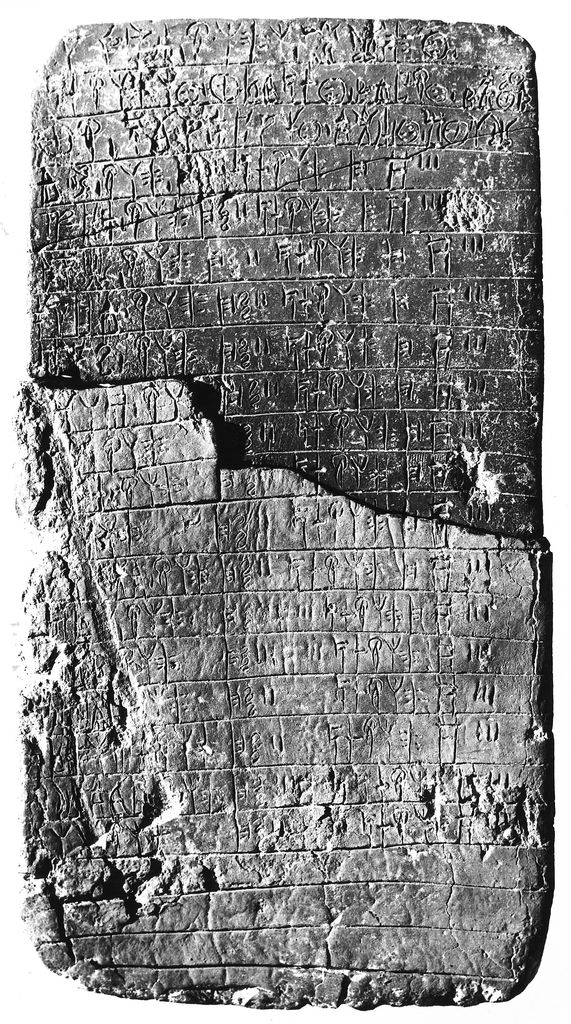
\includegraphics[width=0.35\textwidth]{Images/5072.png} % Adjust width and filename
  \caption{Picture of the original document PY Jn 829.}
  \label{fig:doc4}
\end{figure}

\subsubsection{KN So 4439}
This very short document is an inventory for wheels.
Despite its brevity, it is actually one of the most challenging documents, due to the presence of misleading words.
Tselentis provides the translation for the entire document. \\
\textbf{Linear B text}: \textit{a-mo-ta e-ri-ka te-mi-dwe-ta ROTA ZE 3 MO ROTA 1} \\
\textbf{Greek translation}: \textgreek{ἁρμότα ἑλίκαι τερμιδfέντα: τροχοί ζεύγη 3, μόνος τροχός 1.} \\
\textbf{English translation}: Chariot fittings, willow (wood), rimmed: 3 pairs of wheels, 1 single wheel.

\paragraph{Analysis.}
The analysis of this document is particularly important, as it highlights the challenges posed by certain words that can easily mislead the LLM.
The main terms in this document are:
\begin{itemize}
  \item \textlinb{\Ba\Bmo\Bta} (a-mo-ta), "wheels/chariot", from Ancient Greek \textgreek{ἅρμα}, is the nominative plural and subject of the sentence.
  Despite its original meaning as "wheel", in classical Ancient Greek it came to denote the entire chariot.
  \item \textlinb{\Be\Bri\Bka} (e-ri-ka), "willow tree", from Ancient Greek \textgreek{ἑλικτός}, is here used as an adjective to describe the material of the wheels.
  However, the LLM misinterprets it as a noun, translating it as "willow". Moreover, its connection to the concept of "willow" is attested in Linear B, while in classical Ancient Greek \textgreek{ἑλικτός} means "twisted" or "curved".
  \item \textlinb{\Bte\Bmi\Bdwe\Bta} (te-mi-dwe-ta), "rimmed", from Ancient Greek \textgreek{τερμιόεις}, is correctly identified as an adjective by the LLM.
\end{itemize}
The LLM's English translation fails to capture the full meaning of the document, as it misunderstands the subject of the sentence and misinterprets the adjective referring to the material of the wheels.
Here I report an improved version of the translations, highlighting in red the adjustments and in blue the actual mistakes. \\
\textbf{Greek translation}: \textcolor{red}{\textgreek{ἅρματα}} \textcolor{blue}{\textgreek{ἑλικά}} \textcolor{red}{\textgreek{τερμιοέντα}}\textgreek{: τροχοί ζεύγη 3, μόνος τροχός 1.} \\ 
\textbf{English translation}: \textcolor{blue}{Wheels made of willow tree}, rimmed: 3 pairs of wheels, 1 single wheel.

\begin{figure}[H]
  \centering
  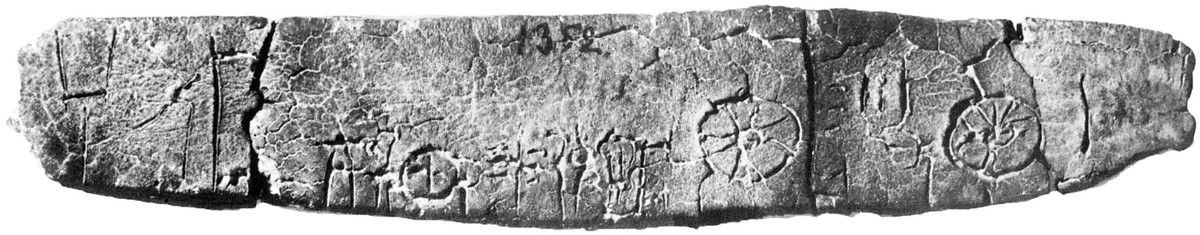
\includegraphics[width=0.7\textwidth]{Images/568.png} % Adjust width and filename
  \caption{Picture of the original document KN So 4439.}
  \label{fig:doc5}
\end{figure}

\subsubsection{KN Sd 4404}
This document is another inventory, this time for chariots.
Due to its fragmentary state, reconstructing its content is quite challenging.
Tselentis provides a translation for only the last fragment of the document. \\
\textbf{Linear B text}: jo [...] i-qo-e-qe wi-ri-ni-jo o-po-qo ke-ra-ja-pi o-pi-i-ja-pi CUR [...] \textit{i-qi-ja [...] ku-do-ni-ja mi-to-we-sa-e a-ra-ro-mo-te-me-na} po-ni-ki-ja BIG 1 \\
\textbf{Greek translation}: \textgreek{[...], ἱππο-ε-κες τε fίρινιοι ὀπωπω κεραίαφι ὀπίαιφι ΔΙΦΡΟΣ. [...] ἱππία Κυδωνία μιλτόfεσσα ἀραρμοτhεμένη φοινικία ΔΙΦΡΟΣ 1.} \\
\textbf{English translation}: [...], and horse-equipped (parts), leathern eye-guards, with horn-like parts, with reins, a chariot. [...] A Cydonian, red-painted, fitted, red-dyed chariot: 1 chariot.

\paragraph{Analysis.}
Overall, the LLM performs well in recognizing the main words in the document, despite its fragmentary condition.
The main terms in this document are:
\begin{itemize}
  \item \textlinb{\Bi\Bqo\Be\Bqe} (i-qo-e-qe), which is linked to \textgreek{ἵππος} "horse". 
  It presents a strange \textit{-e} ending, and is interpreted as "horse-equipped parts", despite the fact that \textit{-qe} is usually a conjunction meaning "and".
  The peculiar ending might be dual ending, but this is only my speculation.
  \item \textlinb{\Bwi\Bri\Bni\Bo} (wi-ri-ni-jo) derives from \textgreek{ῥινός}, "leather", and it is an adjective associated with \textlinb{\Bo\Bpo\Bqo} (o-po-qo), "eye-guards", from \textgreek{ἐπί} and the root \textgreek{ὀπ-}, linked to sight, as in \textgreek{ὄψις}, "sight".
  \item \textgreek{κεραίαφι} (ke-ra-ja-pi) and \textgreek{ὀπίαιφι} (o-pi-i-ja-pi) are both in the instrumental terms, as indicated by the suffix \textit{-pi}, and mean "with horn-like parts" and "with reins", from Ancient Greek \textgreek{κέρας} "horn" PALLE PALLE..., respectively.
\end{itemize}

\subsubsection{PY An 657}
PALLE PALLE...

\subsubsection{PY TA 641}
This document is a short inventory of vessels, in particular tripods and pithoi (large storage jars).
The translation provided by Tselentis covers the first portion of the document, while the rest is left untranslated. \\

\textbf{Linear B text}: \textit{ke-re-ha *201VAS [...] ti-ri-po-de ai-ke-u ke-re-si-jo we-ke *201VAS 2 ti-ri-po e-me po-de o-wo-we *201VAS 1 ti-ri-po ke-re-si-jo we-ke a-pu ke-ka-u-me-no} [...] qe-to *203VAS 3 di-pa me-zo-e qe-to-ro-we *202VAS 1 di-pa-e me-zo-e ti-ri-o-we-e *202VAS 2 di-pa me-wi-jo qe-to-ro-we *202VAS 1 di-pa me-wi-jo ti-ri-jo-we *202VAS 1 di-pa me-wi-jo a-no-we *202VAS 1
\textbf{Greek translation}: σκελέα *201VAS [...] τρίποδες Αἰγεύς Κρήσιον fέργον *201VAS 2, τρίπους ἐνι ποδεί οfωfεις *201VAS 1, τρίπους Κρήσιον fέργον ἀπὸ κεκαυμένος [...], πίθοι *203VAS 3, δέπας μεῖζον τετρόfες *202VAS 1, δέπαε μείζοε τριόfεε *202VAS 2, δέπας μεῖον τετρόfες *202VAS 1, δέπας μεῖον τριόfες *202VAS 1, δέπας μεῖον ἄνοfες *202VAS 1
\textbf{English translation}: Vessels with legs (tripods): [...] two tripods, Cretan work by Aigeus; one tripod, on a foot, with handles; one tripod, Cretan work, burnt off [...]; three pithoi (jars); one larger four-handled cup; two larger three-handled cups; one smaller four-handled cup; one smaller three-handled cup; one smaller cup without handles.

\paragraph{Analysis.}
In this document, the main problem is the positioning of the first two words, which are collocated ad the beginning of the document, but should probably be appended at the end of the first line.
They have been added on top-right of the first row, as the scribe probably ran out of space to complete the sentence.
This mistake was clearly inherited by the translation.
The LLM correctly identifies the main words in the document:
RERUN THIS AS WELL! 

\subsubsection{PY Er 312}

\textbf{Linear B text}: jo [...] i-qo-e-qe wi-ri-ni-jo o-po-qo ke-ra-ja-pi o-pi-i-ja-pi CUR [...] i-qi-ja [...] ku-do-ni-ja mi-to-we-sa-e a-ra-ro-mo-te-me-na po-ni-ki-ja BIG 1,"[...], ἱππο-ε-κες τε fίρινιοι ὀπωπω κεραίαφι ὀπίαιφι ΔΙΦΡΟΣ. [...] ἱππία Κυδωνία μιλτόfεσσα ἀραρμοτhεμένη φοινικία ΔΙΦΡΟΣ 1.","[...], and horse-equipped (parts), leathern eye-guards, with horn-like parts, with reins, a chariot. [...] A Cydonian, red-painted, fitted, red-dyed chariot: 1 chariot.","Grammatical analysis: The document is fragmented, indicated by `[...]`. The initial `jo` is incomplete and cannot be fully translated. `i-qo-e-qe` is interpreted as `ἱππο-ε-κες τε` (horse-equipped and), where `ἱππο-ε-κες` is an adjective (neuter plural, referring to implied parts) and `-qe` is the conjunction 'and'. `wi-ri-ni-jo o-po-qo` translates to `fίρινιοι ὀπωπω` (leathern eye-guards), with `fίρινιοι` (adjective, neuter plural) modifying `ὀπωπω` (noun, neuter plural). `ke-ra-ja-pi o-pi-i-ja-pi` are `κεραίαφι ὀπίαιφι` (with horn-like parts, with reins), both nouns in the instrumental plural (suffix `-pi`). `CUR` is the logogram for `ΔΙΦΡΟΣ` (chariot). The second part of the document describes a specific chariot: `i-qi-ja` is `ἱππία` (chariot), a feminine singular noun. `ku-do-ni-ja` is `Κυδωνία` (Cydonian), an adjective derived from the toponym Cydonia, feminine singular, agreeing with `ἱππία`. `mi-to-we-sa-e` is `μιλτόfεσσα` (red-painted), an adjective, feminine singular, agreeing with `ἱππία`; the final `-e` is a common Linear B simplification. `a-ra-ro-mo-te-me-na` is `ἀραρμοτhεμένη` (fitted), a perfect passive participle, feminine singular, agreeing with `ἱππία` (adapted from the provided neuter plural option to ensure grammatical agreement). `po-ni-ki-ja` is `φοινικία` (red-dyed), an adjective, feminine singular, agreeing with `ἱππία`. `BIG 1` is the logogram for `ΔΙΦΡΟΣ` (chariot) with the numeral 1. 

\subsubsection{KN Fp 1+31}
This document records oil offerings made in the month of Deukios.
In this case, Tselentis provides a translation covering the whole document. \\
\textbf{Linear B text}: \textit{de-u-ki-jo-jo me-no di-ka-ta-jo di-we OLE S 1 da-da-re-jo-de OLE S 2 pa-de OLE S 1 pa-si-te-o-i OLE 1 qe-ra-si-ja OLE S 1 [...] a-mi-ni-so pa-si-te-o-i S 1 [...] e-ri-nu OLE V 3 *47-da-de OLE V 1 a-ne-mo i-je-re-ja V 4 to-so OLE 3 S 2 V 2} \\
\textbf{Greek translation}: \textgreek{Δευκίοιο μηνός: Δικταίῳ Διϝεῖ ΕΛΑΙΟΝ S 1. Δαδαλείονδε ΕΛΑΙΟΝ S 2. Πάνδει ΕΛΑΙΟΝ S 1. πασιθεοῖς ΕΛΑΙΟΝ 1. Θηρασίᾳ ΕΛΑΙΟΝ S 1 [...] Ἀμνισός: πασιθεοῖς S 1 [...] Ἐρινύι ΕΛΑΙΟΝ V 3. Οὐδαδε ΕΛΑΙΟΝ V 1. ἀνέμοιο ἱερείᾳ V 4. τόσον ΕΛΑΙΟΝ 3 S 2 V 2.} \\
\textbf{English translation}: In the month of Deukios: To Dictaean Zeus: 1 S unit of oil. To the Daedaleion: 2 S units of oil. To Pandes: 1 S unit of oil. To all gods: 1 unit of oil. To Therasia: 1 S unit of oil. [...] Amnisos: To all gods: 1 S unit (of oil). [...] To Erinys: 3 V units of oil. To Oudade: 1 V unit of oil. To the priestess of the wind: 4 V units (of oil). Total oil: 3 units, 2 S units, 2 V units.

\paragraph{Analysis.}
The translation of this document is quite accurate: the main terms and phrases are correctly rendered, and the overall structure is preserved.
This success largely reflects the document’s highly regular format, which repeats the same pattern several times.

The main words that appear in this document are:
\begin{itemize}
\item \textlinb{\Bde\Bu\Bki\Bjo\Bjo} (de-u-ki-jo-jo) "of Deukios", linked to Ancient Greek \textgreek{Δευκίος}, the name of a month in the Mycenaean calendar.
This reading is confirmed by the following word \textlinb{\Bme\Bno} (me-no) "month", from Ancient Greek \textgreek{μήν}.
\item The recipients of the offerings are all in the dative case.
The first is \textlinb{\Bdi\Bka\Bta\Bjo} \textlinb{\Bdi\Bwe} (di-ka-ta-jo di-we), corresponding to Ancient Greek \textgreek{Ζεύς/Διός} with the epithet \textgreek{Δικταίος}.
The LLM associates this with Mount Dicte in Crete; Tselentis, however, writes simply "Dikatios".
\item \textlinb{\Bda\Bda\Bre\Bjo\Bde} (da-da-re-jo-de) is correctly recognized as a place-name.
The LLM renders it as the more generic "Daedaleion", while Tselentis gives "the city of Daidalos".
\item \textlinb{\BUvi\Bda\Bde} (*47-da-de) is transliterated by the LLM as "Oudade", but the initial syllabogram has no agreed phonetic value in the literature.
\item \textlinb{\Ba\Bne\Bmo} (a-ne-mo) "of the wind", from Ancient Greek \textgreek{ἄνεμος}, is correctly identified as a genitive; however, it is probably better analyzed as plural rather than singular.
\end{itemize}

In light of the above considerations, I report an improved version of both translations, highlighting in red the adjustments. \\
\textbf{Greek translation}: \textgreek{Δευκίοιο μηνός: Δικταίῳ Διϝεῖ ΕΛΑΙΟΝ S 1. Δαδαλείονδε ΕΛΑΙΟΝ S 2. Πάνδει ΕΛΑΙΟΝ S 1.} \textcolor{red}{\textgreek{πάσι θεοῖς}} \textgreek{ΕΛΑΙΟΝ 1. Θηρασίᾳ ΕΛΑΙΟΝ S 1 [...] Ἀμνισός:} \textcolor{red}{\textgreek{πάσι θεοῖς}} \textgreek{[...] Ἐρινύι ΕΛΑΙΟΝ V 3.} \textcolor{red}{\textgreek{*47-δαδε}} \textgreek{ΕΛΑΙΟΝ V 1.} \textcolor{red}{\textgreek{ἀνέμων}} \textgreek{ἱερείᾳ V 4. τόσον ΕΛΑΙΟΝ 3 S 2 V 2.} \\
\textbf{English translation}: In the month of Deukios: To Dictaean Zeus: 1 S unit of oil. To the \textcolor{red}{city of Daidalos}: 2 S units of oil. To Pandes: 1 S unit of oil. To all gods: 1 unit of oil. To Therasia: 1 S unit of oil. [...] Amnisos: To all gods: 1 S unit (of oil). [...] To Erinys: 3 V units of oil. To \textcolor{red}{?-dade}: 1 V unit of oil. To the priestess of the \textcolor{red}{winds}: 4 V units (of oil). Total oil: 3 units, 2 S units, 2 V units.

\begin{figure}[H]
  \centering
  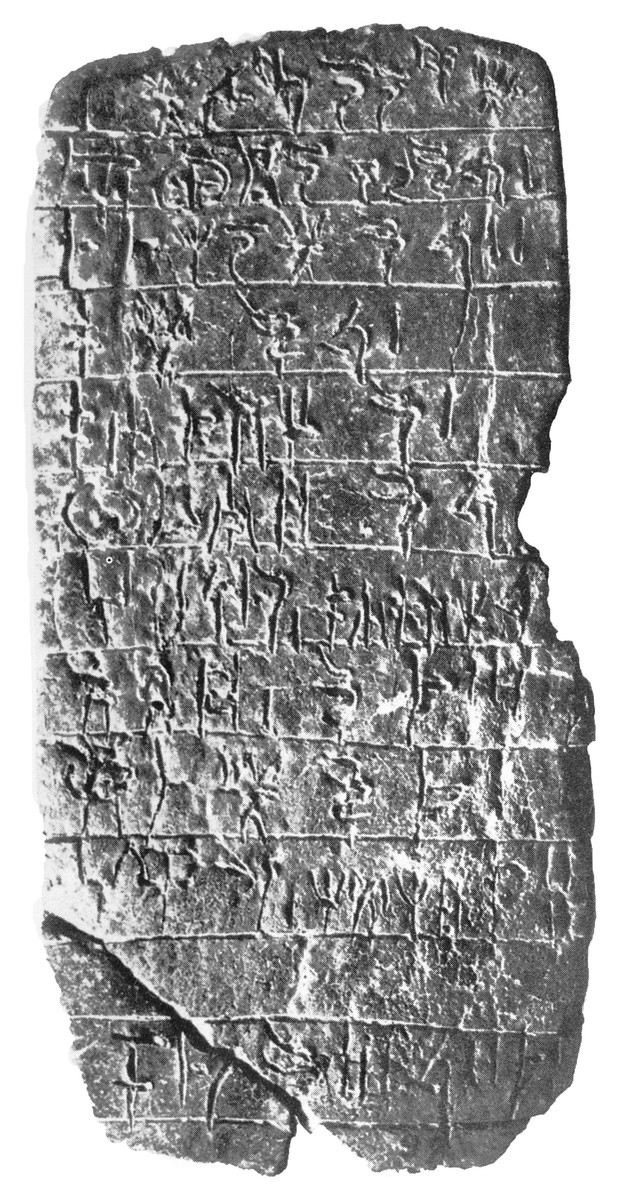
\includegraphics[width=0.4\textwidth]{Images/4088.png} % Adjust width and filename
  \caption{Picture of the original document KN Fp 1+31.}
  \label{fig:doc8}
\end{figure}

\subsubsection{PY Ab 573}
PALLE PALLE...

\subsubsection{PY Un 718}
This last document is an administrative record listing offerings.
The translation provided by Tselentis for this document covers only the first portion. \\
\textbf{Linear B text}: \textit{sa-ra-pe-da po-se-da-o-ni do-so-mo o-wi-de-ta-i do-so-mo to-so e-ke-rya-wo do-se GRA 4 VIN 3 BOSm 1} tu-ryo TU+RYO 10 ko-wo *153 1 me-ri-to V 3 o-da-ha da-mo GRA 2 VIN 2 OVISm 2 TU+RYO 5 a-re-ro A+RE+PA V 2 *153 1 to-so-de ra-wa-ke-ta do-se OVISm 2 me-re-u-ro FAR T 6 VIN S 2 o-da-ha wo-ro-ki-jo-ne-jo ka-ma GRA [...] T 6 VIN S 1 TU+RYO 5 me-ri [...] 1 [...] V 1 \\
\textbf{Greek translation}: \textgreek{Σαραπέδα Ποσειδάωνι δόσμος, ὀfιδέται δόσμος. Τόσος Ἐχελάfων δώσει: σῖτος 4, οἶνος 3, ταῦρος 1, τυρίον TU+RYO 10, κοῦρος *153 1, μέλι V 3. Ὀδαhα δᾶμος: σῖτος 2, οἶνος 2, κρίος 2, τυρίον TU+RYO 5. Ἀρέλος: ἀλείφαρ V 2, *153 1. Τοσόνδε λαfαγέτας δώσει: κρίος 2, ἄλευρον ΦΑΡ T 6, οἶνος S 2. Ὀδαhα fρογιώνειον κᾶμα: σῖτος [...] T 6, οἶνος S 1, τυρίον TU+RYO 5, μέλι [...] 1 [...] V 1.} \\
\textbf{English translation}: Sarapeda: an offering to Poseidon, an offering to the overseers. So much Echelāwōn will give: 4 units of grain, 3 units of wine, 1 bull, 10 units of cheese (TU+RYO), 1 boy (*153), 3 'V' units of honey. Also, the community: 2 units of grain, 2 units of wine, 2 rams, 5 units of cheese (TU+RYO). Arelos: 2 'V' units of ointment (A+RE+PA), 1 unit of *153. So much the Lawagetas will give: 2 rams, 6 'T' units of flour (FAR), 2 'S' units of wine. Also, Wrogion's plot: [...] 6 'T' units of grain, 1 'S' unit of wine, 5 units of cheese (TU+RYO), [...] 1 'V' unit of honey.

\paragraph{Analysis.}
The LLM provides a fairly accurate translation of this document, with some problematic issues.
\begin{itemize}
  \item The first word \textlinb{\Bsa\Bra\Be\Bpe\Bda} (sa-ra-pe-da) is transliterated as "Sarapeda". The LLM considers it as a proper noun or a toponym. Its possible toponym function is mentioned also by Chadwick and Ventris in their lexicon \cite{chadwick-notes}.
  However, Tselentis interprets it as an epithet of Poseidon, appearing as the next word \textlinb{\Bpo\Bse\Bda\Bo\Bni} (po-se-da-o-ni), linked to Ancient Greek \textgreek{Ποσειδῶν}, translating it as "Srapedas".
  \item The word \textlinb{\Bo\Bwi\Bde\Bta\Bi} (o-wi-de-ta-i) is clearly linked to Ancient Greek \textgreek{οἶδα} "to know". Tselentis mentions that it is a religious title, while the LLM tries to interpret it as "overseers". However, it is correctly identified as a dative plural.
  \item The verb \textlinb{\Bdo\Bse} (do-se) is correctly identified as the 3rd person singular future active indicative of \textgreek{δίδωμι}, "to give".
  \item The most notable feature of the enumnerated items in this fragment is the presence of logographic merging of common linear B words, which the LLM was able to reconsturct.
  For example, the word \textlinb{\Btu\Broii} (tu-ryo) appears both isolated and merged into a unique symbol (TU+RYO), representing "cheese" from Ancient Greek \textgreek{τυρίον}. 
  Moreover, \textlinb{\Ba\Bre\Bpa} (a-re-pa) appears uniquely as a logogram (A+RE+PA), representing "ointment" from Ancient Greek \textgreek{ἀλείφαρ}.

\end{itemize}

Grammatical analysis: The document is an administrative record detailing offerings and distributions. `sa-ra-pe-da` (Σαραπέδα) is a proper noun in the nominative, likely acting as a heading or subject. `po-se-da-o-ni` (Ποσειδάωνι) is a theonym in the dative case, indicating the recipient. `do-so-mo` (δόσμος) is interpreted as a noun (offering/gift) in the nominative case, despite the classifier indicating 'verb', as it fits the administrative context of lists of offerings. `o-wi-de-ta-i` (ὀfιδέται) is a noun in the dative plural, indicating recipients. `to-so` (τόσος) and `to-so-de` (τοσόνδε) are adjectives meaning 'so much/so many', introducing the quantities to be given, with `-de` as an allative/demonstrative suffix on the latter. `e-ke-rya-wo` (Ἐχελάfων), `da-mo` (δᾶμος), `a-re-ro` (Ἀρέλος), and `ra-wa-ke-ta` (λαfαγέτας) are proper nouns or titles in the nominative case, acting as subjects or headings for their respective entries. `do-se` (δώσει) is the 3rd person singular future active indicative of `δίδωμι` (to give). `tu-ryo` (τυρίον), `ko-wo` (κοῦρος), `me-ri` (μέλι), `me-re-u-ro` (ἄλευρον), `ka-ma` (κᾶμα), and `A+RE+PA` (ἀλείφαρ) are nouns in the nominative/accusative case, representing the items being listed. `me-ri-to` is interpreted as `μέλι` (honey) in the nominative/accusative, as it's part of a list of items, overriding the genitive form `μέλιτος` or the thematic -o classifier. `o-da-ha` (ὀδαhα) is an adverb meaning 'also' or 'thus', introducing subsequent entries. `wo-ro-ki-jo-ne-jo` (fρογιώνειον) is an adjective modifying `ka-ma` (κᾶμα), indicating a plot belonging to or associated with Wrogion. Logograms (GRA, VIN, BOSm, OVISm, TU+RYO, FAR, A+RE+PA, *153) and units (T, S, V) are treated as direct representations of commodities and their quantities. Logical/Syntactic analysis: The document is structured as a series of administrative entries, typical of Linear B tablets. The initial line acts as a general heading or summary of offerings. Subsequent sections follow a pattern: `[Giver/Entity] [Verb (will give, or implied)] [List of items and quantities]`. The phrases introduced by `o-da-ha` (also) indicate additional entries or distributions from different entities. The use of `to-so` and `to-so-de` emphasizes the total quantity of items to be given by specific individuals or groups. The lists of items are paratactic, with quantities following the logograms. Subordinate clause analysis: No explicit subordinate clauses are present. The structure is primarily paratactic, listing entities, actions, and items. Error recovery: The discrepancy in `do-so-mo` (classified as verb, but options are nouns) and `me-ri-to` (classified as thematic in -o, but `μέλι` is athematic and `μελιτος` is genitive) was resolved by prioritizing semantic coherence within the administrative context, interpreting them as nouns (offering, honey) in the appropriate case for a list."

